% this file is called up by thesis.tex
% change according to folder and file names
\ifpdf
    \graphicspath{{6/figures/PNG/}{6/figures/PDF/}{6/figures/}}
\else
    \graphicspath{{6/figures/EPS/}{6/figures/}}
\fi

%: ----------------------- contents from here ------------------------
% content in this file will be fed into the main document

\chapter{Optimization of a Compressor Annular Cascade} % top level followed by section, % ---------------------------------------------------------------------------


%\begin{flushright}
%I love the smell of turbines in the morning.
%\linebreak
%Lynn Kilgore
%\end{flushright}

In this chapter, the design-optimization of a stationary compressor annular cascade is presented. This case is used to assess the performance of the proposed M(PCA)AEA(PCA), as described in Chapter \ref{VarCorrChapter}, and compare it with the MAEA developed in the framework of previous PhD theses \cite{phd_Kampolis,phd_Giotis,phd_Karakasis} at PCOpt/LTT/NTUA. The same optimization problem was studied in \cite{phd_Kampolis} and is now revisited with the newly developed M(PCA)AEA(PCA). 

The annular compressor annular cascade this chapter is dealing with has been installed at LTT/NTUA where both measurements  \cite{phd_doukelis,mathiou97}  and CFD computations \cite{politis98a} have been performed in the past. The cascade geometry was designed by SNECMA for investigating tip-clearance effects at high Mach numbers \footnote{Experimental measurements on this cascade were performed in the framework of the project entitled ``Advanced Civil Core Compressor Aerodynamics'', funded by the European Commission, AER2-CT92-0039, 1/1/1993-30/9/1996.}. This geometry is considered to be the reference one, throughout this chapter. 

\begin{figure}[h!]
\centering
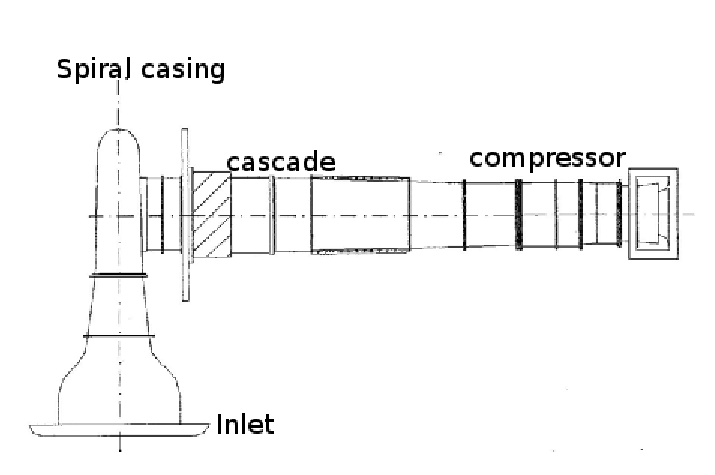
\includegraphics[width=.8\textwidth]{experim.eps}
\caption{Optimization of a compressor annular cascade. Experimental set-up.}
\label{ntua_blade.experim}
\end{figure}


The evaluation software solves the Navier-Stokes equations for compressible flows through a time-marching, vertex-centered, finite volume method on unstructured hybrid grids. The aforementioned software was developed and validated at PCOpt/LTT/NTUA \cite{phd_Vera,phd_Kampolis}. The convection terms are discretized via the Roe scheme \cite{Roe81}. Second-order spatial accuracy is achieved through the MUSCL interpolation \cite{vleer:muscl} along with the van Leer--van Albada limiting function \cite{valbada:82}. 

The Navier-Stokes solver employed the high-Reynolds variant of the Spalart-Allmaras turbulence model \cite{phd_Kampolis}. Since wall functions were used, the grid was coarse enough, in order to reduce as much as possible the CPU cost per evaluation. For all candidate blade shapes, grids of $\backsim \! 600.000$ nodes were generated from scratch, using an automated grid generation tool \cite{phd_Kampolis}. In general, any of these grids comprises $\backsim \! 225.000$ tetrahedra, $\backsim \! 6.000$ pyramids, $\backsim \! 200.000$ prisms and $\backsim \! 400.000$ hexahedrals. The average distance of the first nodes off the wall was $\backsim \! 5\times10^{-5}m$ and the total time of grid generation was $\backsim \! 11$ minutes on a modern single-core processor. 

At the inlet, total pressure and temperature profiles along with the radial distributions of the peripheral and radial velocity flow angles were imposed as boundary conditions. At the exit, the static pressure at the hub was imposed and the pressure distribution over the exit plane was continuously updated by means of the radial equilibrium equation. 
Each CFD evaluation was carried out in parallel, by partitioning the unstructured grid into $8$ equally-loaded sub-domains with the minimum interface between them so as to minimize the communication overhead. Running on an eight-core node the cost per CFD evaluation (excluding grid generation) is approximately $1.2$ hours. 


%Boundary conditions are: 
%\begin{itemize}
%	\item{\textbf{Inlet:}} 
%	\begin{itemize}
%		\item Radial distribution of total pressure.
%		\item Radial distribution of temperature.
%		\item Radial distribution of velocity direction (angles in peripheral and radial direction).
%		\item turbulence intensity (here $1.5\%$).  
%	\end{itemize}    
%	\item{\textbf{Outlet:}} 
%	\begin{itemize}
%		\item Static pressure at hub.
%		\item Radial equilibrium.
%	\end{itemize}    
%\end{itemize}



\begin{figure}[h!]
\centering
  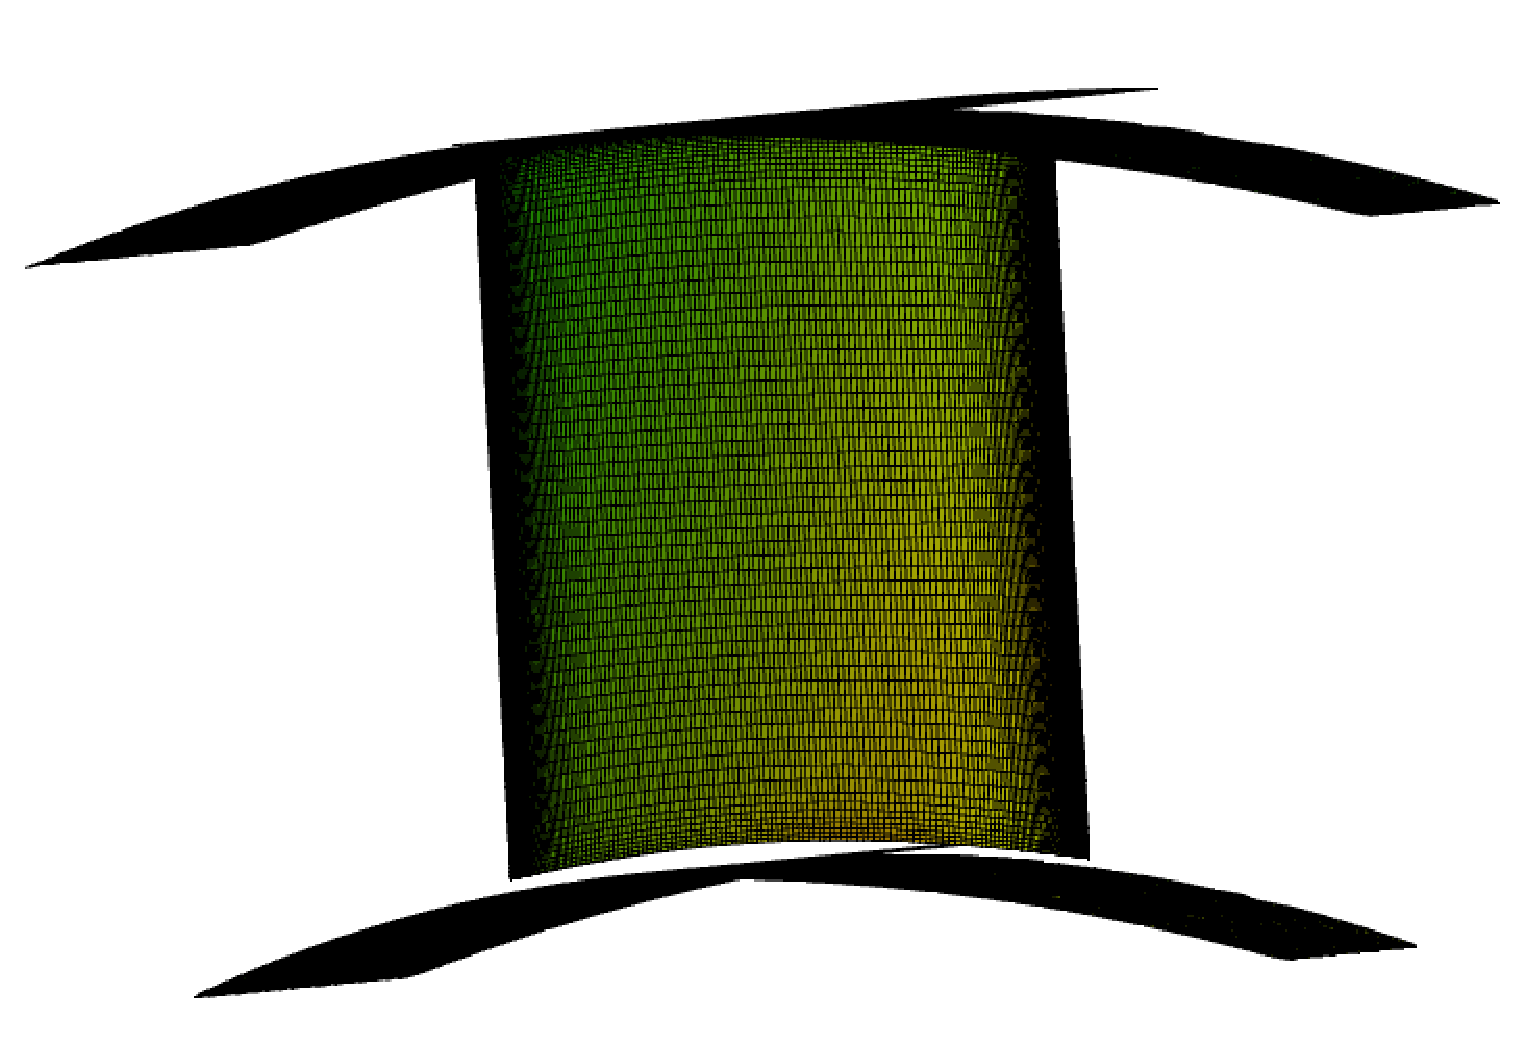
\includegraphics[width=.7\textwidth]{blade.eps}
  \caption{Optimization of a compressor annular cascade. The cascade blades are fixed at the shroud, forming the tip-clearance close to the stationary hub. Chord is equal to $C=0.1m$ and tip-clearance height is equal to $0.02C$}
  \label{res:ntua_blade:blade}
\end{figure}

\section{Blade Shape Parameterization}
Since the blade airfoil shape is identical along the spanwise direction, the parameterization of a single airfoil is enough for the entire blade shape. Non-Uniform-Rational-B-Splines (NURBS) are used to control both airfoil sides. To parameterize the suction or the pressure side, $15$ control points were used. Among them, $5$ were free to change and, given that each control point has two degrees of freedom (its two coordinates), the number of design variables was $5 \! \times \! 2$ for the each side, yielding thus $20$ degrees of freedom in total, \cite{phd_Kampolis}. 

\begin{figure}[h!]
\centering
  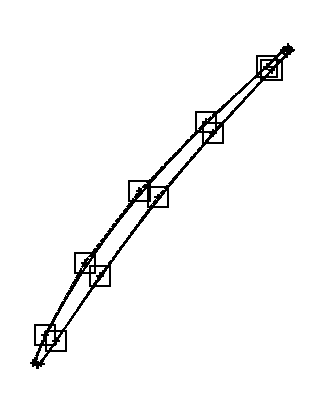
\includegraphics[width=.5\textwidth]{foil_cp2.eps}
  \caption{Optimization of a compressor annular cascade. The $20$ design variables used for the design-optimization of the compressor annular cascade airfoil, \cite{phd_Kampolis}. Boxes demonstrate the variable range for each design variable i.e. the space that each free control point may lay in. NURBS control point without a corresponding box are the ($10$ per side) fixed control points which are located at the leading and trailing edge region.}
  \label{res:ntua_blade:cp}
\end{figure}



\section{Case Presentation}

The results of the two different optimization runs, with the same $20$ design variables each are presented in order to demonstrate the gains offered by the use of the methods proposed in Chapter \ref{VarCorrChapter}.  
The first optimization run was carried out using the ``standard'' MAEA (i.e. the one presented in previous PhD theses carried out at PCOpt/LTT/NTUA, \cite{phd_Karakasis,phd_Kampolis}) with $\mu\!=\!20$, $\lambda\!=\!60$ and $\lambda_e\!=\!4$. The IPE phase started once the first $220$ individuals were stored in the DB. Metamodels, i.e. RBF networks, were trained on a number of already evaluated patterns which varied between $20$ and $30$; all training patterns were defined in $\Re^{20}$. The second optimization was based on the proposed M(PCA)AEA(PCA) method, with the same population sizes with the corresponding MAEA. In this run, RBF networks were trained on a much smaller number of training patterns (between $5$ and $8$) and all of the training patterns were defined in the $\Re^{10}$ space. In this case, due to the reduced dimension, the IPE phase started earlier, just after the first $150$ individuals were stored in the DB.     

   
\subsection{Objectives and Constraints}
The optimization problem was solved with a single objective, i.e.\ aiming at the minimization of the spanwise-averaged pressure loss coefficient
$PLC_{av}$. The $PLC_{av}$ value results from the averaging (in spanwise direction) of the $PLC(r)$ distribution (computed at each radial position). The latter is defined as     
\begin{equation}
PLC(r)=\frac{p_{t,inl}-p_t(r)}{p_{t,inl}-p_{inl}}
\label{res:ntua_blade:plc}
\end{equation}

Furthermore, the cascade to be designed must respect aerodynamic and geometrical constraints. The aerodynamic one requires that the minimum average outlet flow angle should not exceed $53^o$, namely $\alpha_2<53^o$. The reference blade of the compressor annular cascade installed at LTT/NTUA gives $\alpha_2\!=\!52.12^o$. Geometrical constraints were used to make the blade respect the desirable minimum airfoil thickness at three positions, namely at $30\%$, $~60\%$ and $90\%$ of chord. The minimum allowed thickness values were set to the $90\%$ of the corresponding reference values.      


\section{Results}

Fig.\ \ref{PCAcomp} demonstrates the evolution of the objective function ($PLC_{av}$) values in terms of the number of evaluations for the MAEA and M(PCA)AEA(PCA). In fig.\ \ref{PCAcomp2}, the effects of the use of PCA during the metamodel training phase (earlier start and higher accuracy) is shown. The use of PCA during the application of the evolution operators further increases EA's efficiency (fig. \ref{PCAcomp}). With the help of PCA, in order to guide both the metamodels and the evolution operators, the  M(PCA)AEA(PCA) reached the $PLC_{av}$ value of $0.104$ at $\backsim 250$ evaluations. MAEA needed $\backsim 500$ evaluations to reach the same level of $PLC_{av}$.      


\begin{figure}[h!]
\begin{minipage}[b]{1\linewidth}
 \centering
 \resizebox*{11cm}{!}{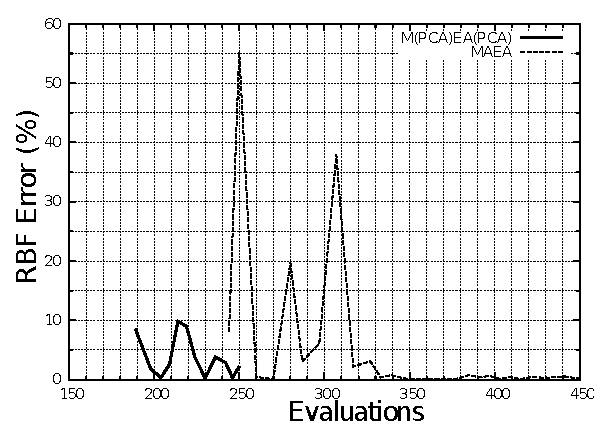
\includegraphics{Comp2.eps}}
\end{minipage}
\caption{Optimization of a compressor annular cascade. Comparison of the metamodel (RBF) prediction error during the evolution, working either with MAEA or M(PCA)AEA(PCA). Since, in M(PCA)AEA(PCA), metamodels start being used earlier, the continuous line is shifted ahead.} 
\label{PCAcomp2}
\end{figure}

\begin{figure}[h!]
\begin{minipage}[b]{1\linewidth}
 \centering
 \resizebox*{11cm}{!}{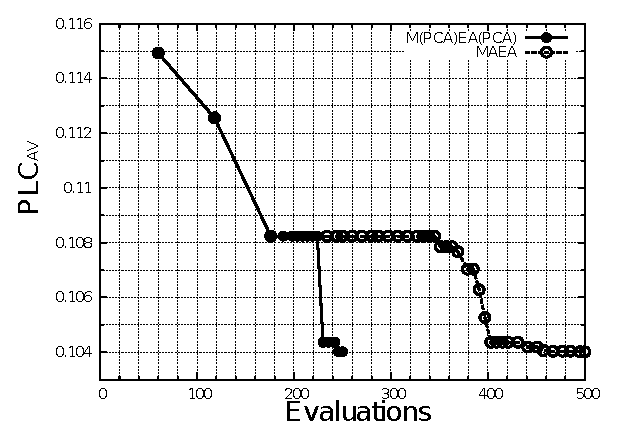
\includegraphics{Comp.eps}}
\end{minipage}
\caption{Optimization of a compressor annular cascade. Comparison of the performance of MAEA and M(PCA)AEA(PCA).} 
\label{PCAcomp}
\end{figure}




The optimal airfoil shape computed using M(PCA)AEA(PCA) has $PLC_{av}=0.104$ and is shown in fig.\ \ref{res:ntua_blade:final}. This design respects all geometrical and aerodynamic constraints and its outlet flow angle is $\alpha_2=52.6^o$   


\begin{figure}[h!]
\centering
  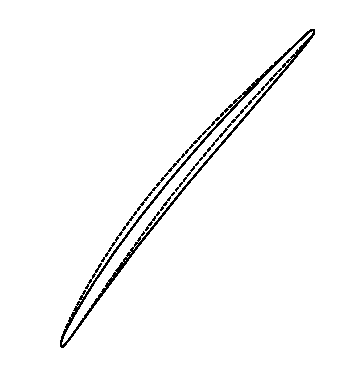
\includegraphics[width=.7\textwidth]{ntua_foils.eps}
  \caption{Optimization of a compressor annular cascade. The optimal blade airfoil shape computed using the M(PCA)AEA(PCA) (continuous line), compared with the reference one (dashed line).}
  \label{res:ntua_blade:final}
\end{figure}

%Finally the pressure contour of the optimal blade is presented in figure \ref{res:ntua_blade:Optimal}.

%\begin{figure}[h!]
%\centering
%  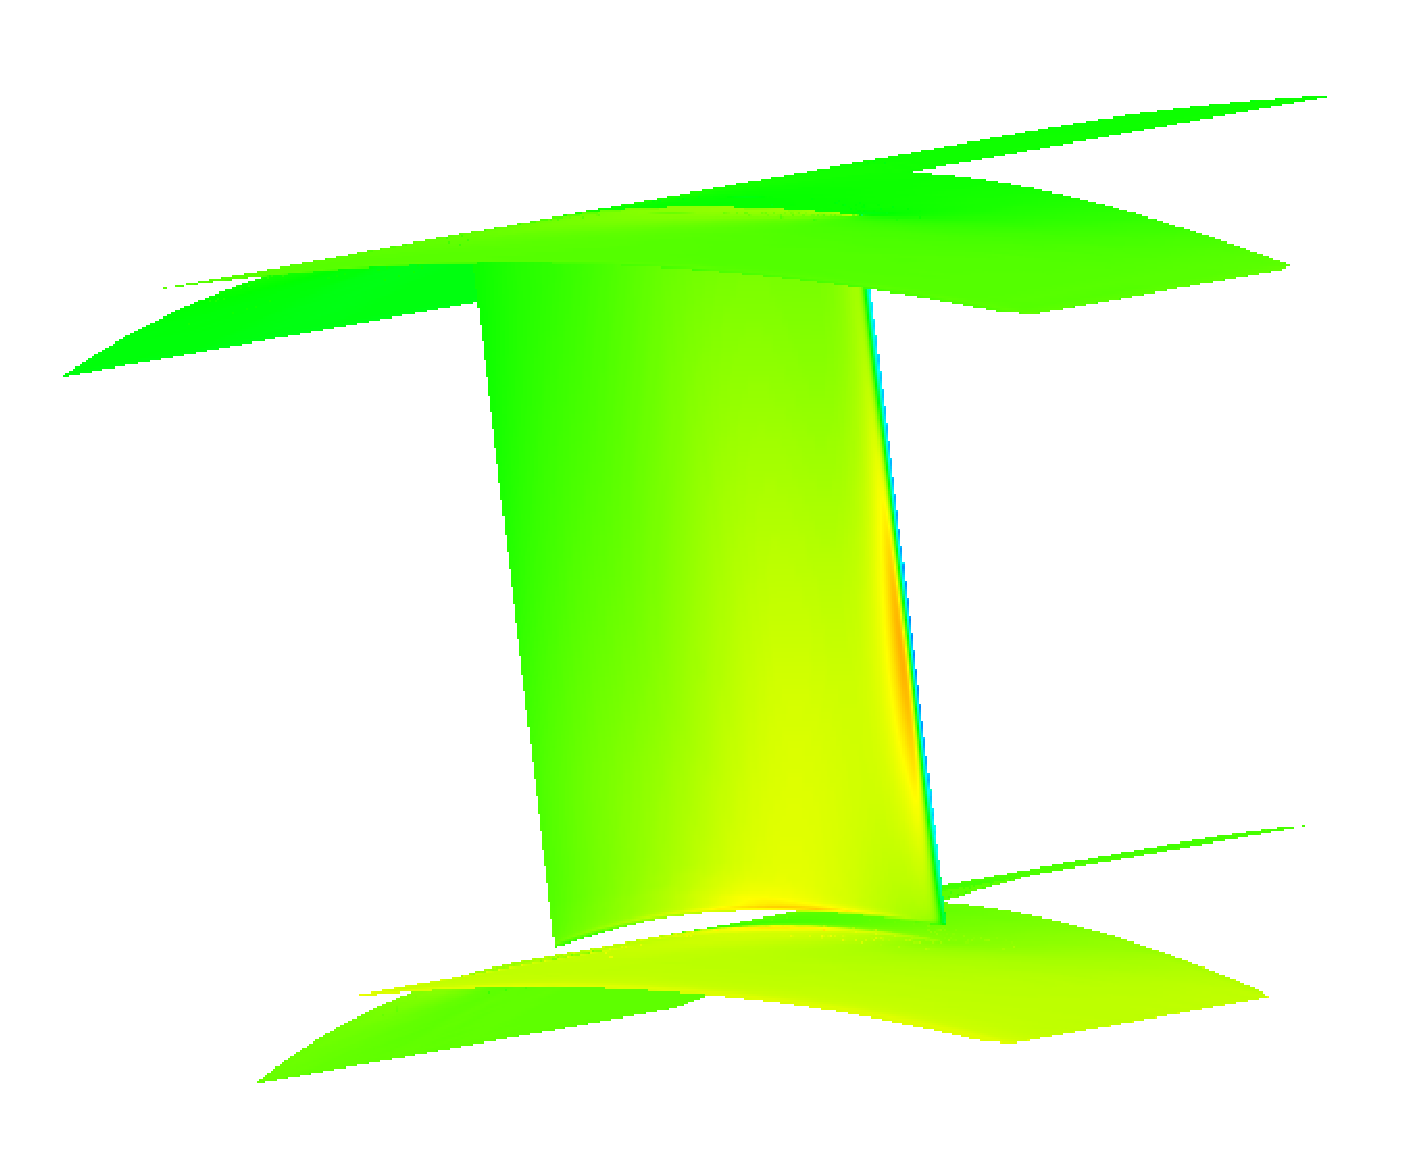
\includegraphics[width=.9\textwidth]{Optimal.eps}
%  \caption{Optimization of a compressor annular cascade: Pressure contour over the optimal design.}
%  \label{res:ntua_blade:Optimal}
%\end{figure}

% ----------------------- end of thesis sub-document ------------------------
% ---------------------------------------------------------------------------
